
%% !TEX root = manual.tex

\begin{figure}[h!]
\centering
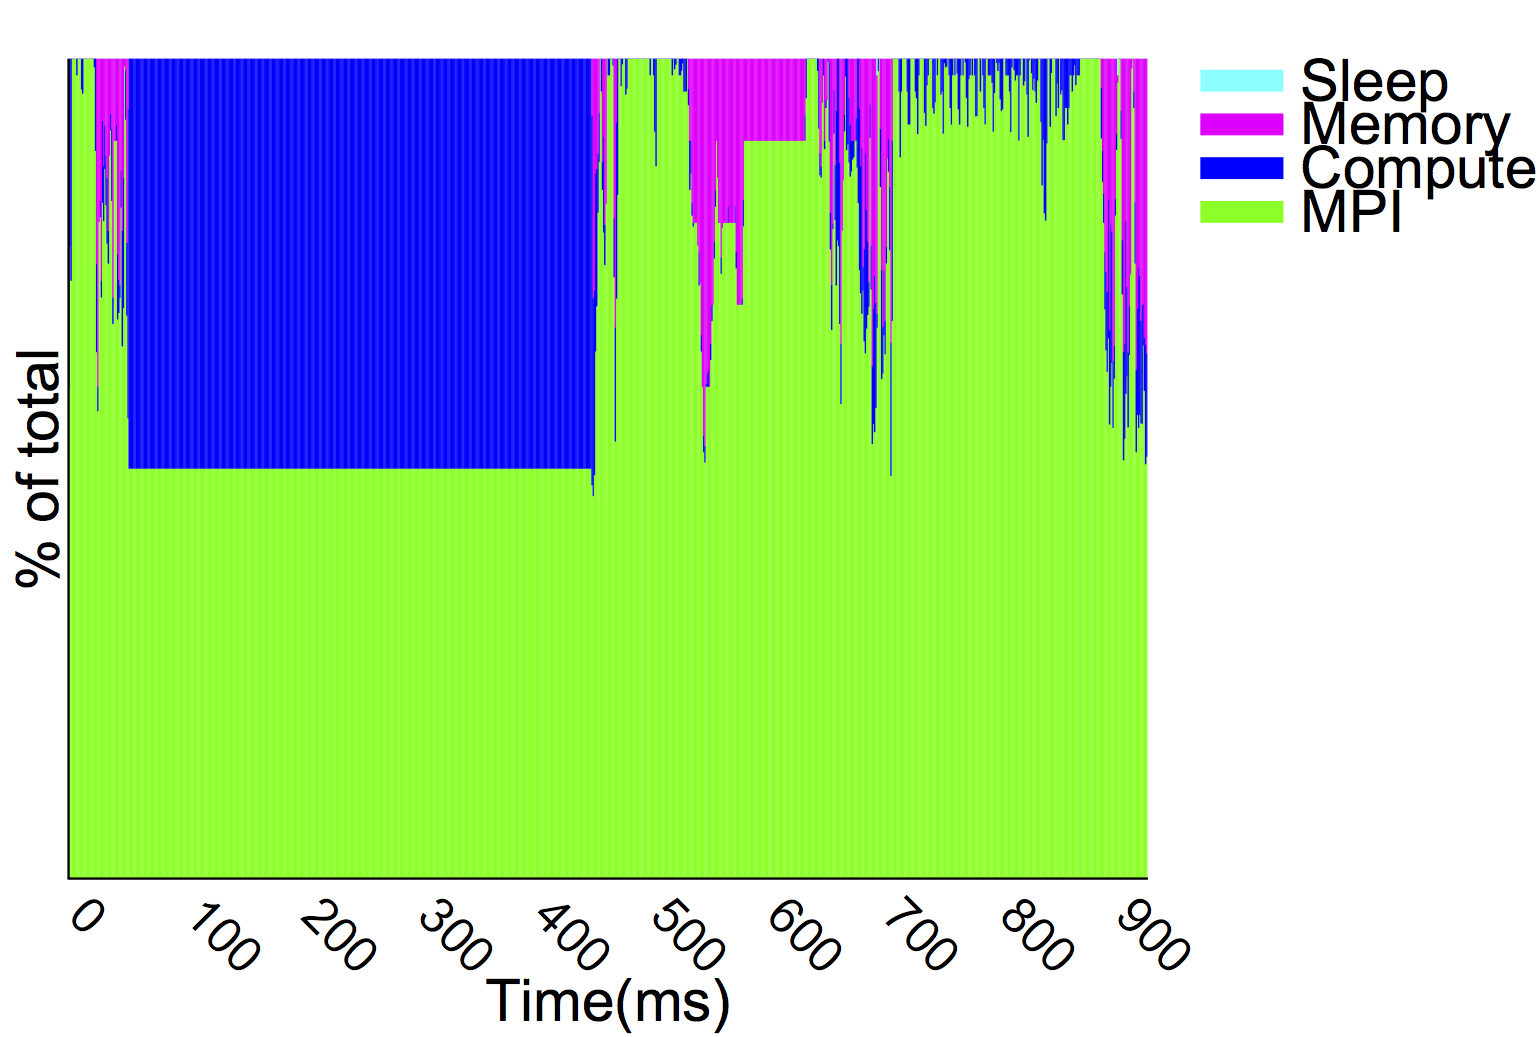
\includegraphics[width=0.6\textwidth]{figures/gnuplot/ftq/ftq.png}
\caption{Application Activity (Fixed-Time Quanta; FTQ) for Simple MPI Test Suite}
\label{fig:ftq}
\end{figure}
\section{Fixed-Time Quanta Charts}
\label{sec:tutorials:ftq}
Another way of visualizing application activity is a fixed-time quanta (FTQ) chart.
While the call graph gives a very detailed profile of what code regions are most important for the application, they lack temporal information.
The FTQ histogram gives a time-dependent profile of what the application is doing (Figure \ref{fig:ftq}).
This can be useful for observing the ratio of communication to computation.
It can also give a sense of how ``steady'' the application is, 
i.e. if the application oscillates between heavy computation and heavy communication or if it keeps a constant ratio.
In the simple example, Figure \ref{fig:ftq}, we show the FTQ profile of a simple MPI test suite with random computation mixed in.
In general, communication (MPI) dominates.  However, there are a few compute-intensive and memory-intensive regions.

The FTQ visualization is activated by another input parameter

\begin{ViFile}
ftq = <fileroot>
\end{ViFile}

where the \inlinefile{fileroot} parameter gives a unique prefix for the output files. 

After running, two new files appear in the folder: \inlineshell{<fileroot>_app1.p} and \inlineshell{<fileroot>_app1.dat}.
\inlineshell{plot_app1.p} is a Gnuplot script that generates the histogram as a postscript file.

\begin{ShellCmd}
your_project$ gnuplot plot_app1.p > output.ps
\end{ShellCmd}
Gnuplot can be downloaded from \url{http://www.gnuplot.info} or installed via MacPorts.
We recommend version 4.4, but at least 4.2 should be compatible.

The granularity of the chart is controlled by the \inlinefile{ftq_epoch} parameter in the input file. 
The above figure was collected with

\begin{ViFile}
ftq_epoch=5us
\end{ViFile}
Events are accumulated into a single data point per ``epoch.''
If the timestamp is too small, too little data will be collected and the time interval won't be large enough to give a meaningful picture.
If the timestamp is too large, too many events will be grouped togther into a single data point, losing temporal structure.

Using fully namespace parameters, this would be specified as:


\begin{ViFile}
node.os.ftq.fileroot=<fileroot>
node.os.ftq.epoch=5us
\end{ViFile}
